\chapter{Rekabentuk Sistem}\label{c4}

\section{Pengenalan}
Fasa ini merupakan fasa lanjutan hasil dari analisis dan kajian awalan yang telah dilakukan di mana, rekabentuk sistem mula dirangka dan langkah-langkah penyelesaian masalah dilakukan dengan menggunakan pewakilan-pewakilan sama ada rajah, cartalir atau model yang bersesuaian bagi menunjukkan dengan jelas tindakan yang diambil untuk tujuan tersebut.

Proses rekabentuk adalah bertujuan untuk menghasilkan spesifikasi rekabentuk berdasarkan keperluan pengguna dan skop projek. Ini memudahkan kerja-kerja pengekodan dalam peringkat implementasi projek. Gambaran terperinci tentang rekabentuk projek diterangkan dalam seksyen hasil analisis dan rekabentuk ini.

\section{Rekabentuk Sistem}
Rekabentuk ELWI direka untuk memenuhi keperluan mewujudkan antaramuka bergrafik bagi sistem terbenam Linux. Seperti yang telah dijelaskan sebelum ini, antaramuka bergrafik ELWI dibina bagi mempermudah tugas penyelenggara sistem terbenam. Dalam kes ini, penyelenggara boleh ditakrifkan sebagai operator yang mengendalikan sistem terbenam Rain Gauge. Oleh kerana sistem terbenam ini beroperasi secara automatik tanpa operator, antaramuka ELWI hanya akan digunakan oleh operator sistem bagi tujuan penyelenggaraan dan konfigurasi. Rajah \ref{c4:f1} menunjukkan kes guna operator yang menggunakan antaramuka ELWI untuk membuat konfigurasi dan memeriksa sistem terbenam Rain Gauge.

\begin{figure}[!h]
\centering{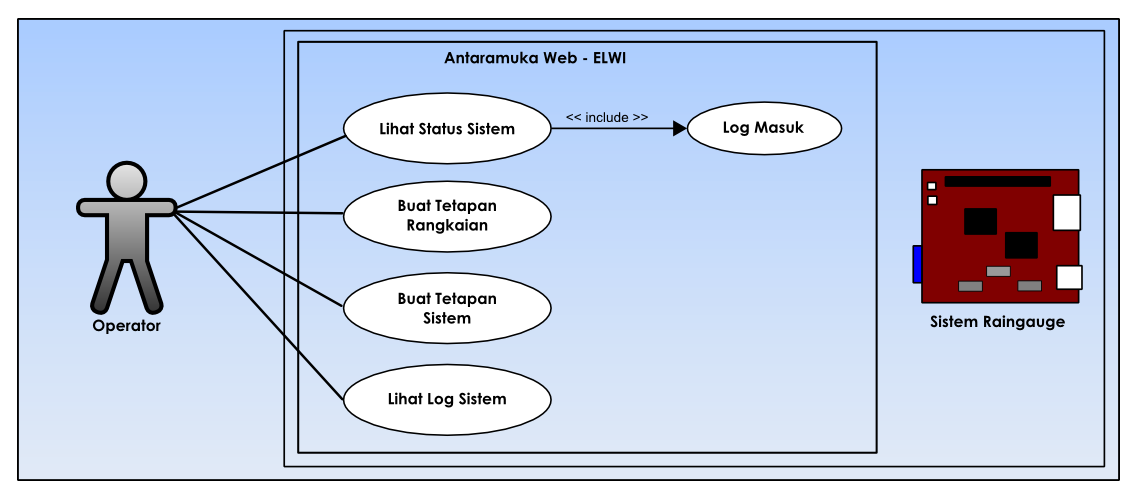
\includegraphics[width=1\textwidth]{source/fig/kes-guna-ELWI.eps}}
\caption[Kes guna untuk Operator sistem]{Kes guna untuk Operator sistem}
\label{c4:f1}
\end{figure}

Dari Rajah \ref{c4:f1}, terdapat satu kes guna melibatkan operator yang ditugaskan untuk membuat konfigurasi dan penyelenggaraan sistem terbenam linux menggunakan antaramuka ELWI. Keterangan mengenai kes guna ini ditunjukkan dalam Jadual \ref{c4:t1}.

\begin{table}[H]
	\centering{
		\newcolumntype{R}{>{\centering}X}%
		\begin{tabularx} {\textwidth} {|>{\setlength\hsize{0.7\hsize}}X|X<{\setlength\hsize{1.3\hsize}}|}
			\hline
			\textbf{Kes Guna} & \textbf{Keterangan} \\ \hline
			Log Masuk & Sebelum operator dapat menggunakan ELWI, beliau perlu log masuk menggunakan katalaluan untuk tujuan keselamatan \\ \hline 
			Lihat Status Sistem & Digunakan untuk melihat status semasa sistem terbenam Rain Gauge. \\ \hline 
			Buat Tetapan Rangkaian & Digunakan untuk membuat konfigurasi rangkaian bagi membolehkannya berhubung dengan pelayan utama dan menghantar data masa nyata. \\ \hline
			Buat Tetapan Sistem & Mengubah tetapan sistem terbenam seperti ID perkakasan supaya dapat dikenalpasti oleh pelayan \\ \hline
			Lihat Log Sistem & Untuk tujuan penyelenggaraan, operator boleh melihat log sistem untuk mengetahui sejarah yang berlaku pada sistem sepanjang ia beroperasi. \\ \hline
		\end{tabularx}
	} 
	\newline \newline
    \caption[Keterangan Kes Guna Operator]{Keterangan Kes Guna Operator}
    \label{c4:t1}
\end{table}

\section{Rekabentuk Antaramuka Pengguna}
Mewujudkan antaramuka pengguna bergrafik merupakan matlamat utama projek ini dilakukan. Rekabentuk antaramuka pada aplikasi membolehkan pengguna berinteraksi dengan aplikasi dengan lebih mudah bagi tujuan yang telah dikhususkan. Antaramuka pengguna yang dibina adalah berkonsepkan antaramuka pengguna bergrafik yang mesra pengguna dan secara tidak langsung ianya lebih interaktif dan amat sesuai untuk pengguna akhir yang memiliki pengetahuan yang minimum mengenai arahan-arahan dalam sistem operasi Linux.

Dalam kajian ini, antaramuka pengguna bergrafik menggunakan teknologi web telah dibina untuk mempermudah dan mempercepatkan tugas konfigurasi sistem terbenam Rain Gauge bagi menggantikan kaedah konfigurasi menggunakan arahan-arahan pada terminal yang perlu dihafal dan diingat oleh operator. Antaramuka web ini mudah diakses menggunakan pelayar web dengan menaip IP perkakasan terbenam. Rajah \ref{c4:f2} menunjukkan antaramuka Login yang menyekat akses umum kepada antaramuka sistem terbenam ini. Oleh yang demikian, hanya operator tertentu yang mempunyai kata laluan sahaja akan dapat mengakses antaramuka web ini.
 
\begin{figure}[!h]
\centering{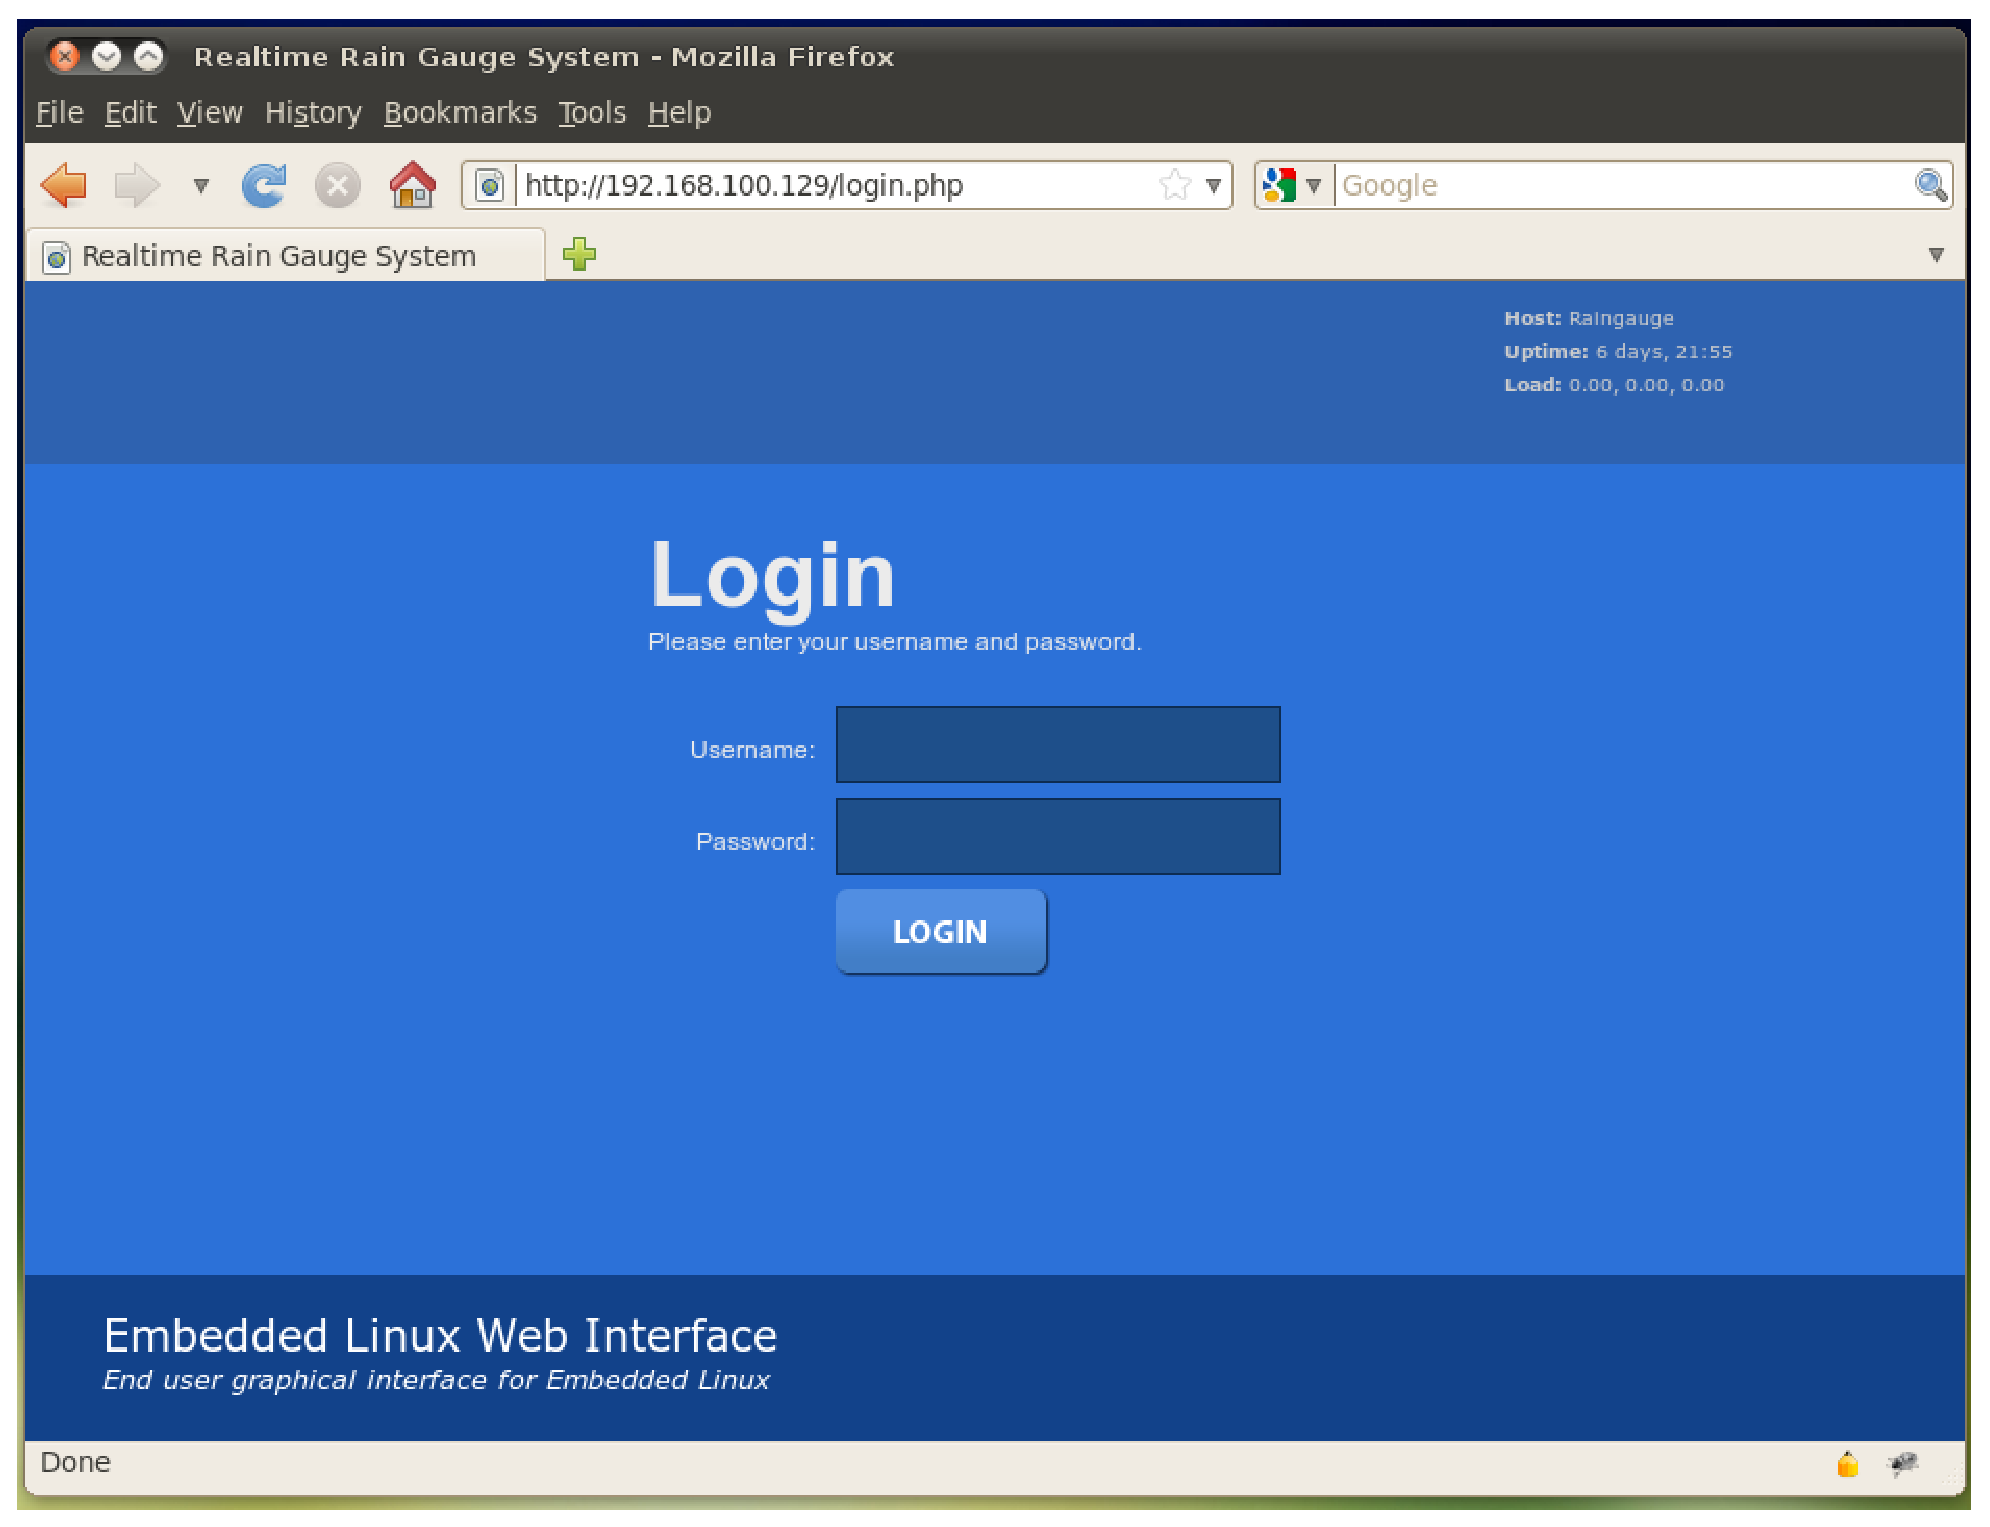
\includegraphics[width=1\textwidth]{source/fig/log-masuk.eps}}
\caption[Antaramuka Login ELWI]{Antaramuka Login ELWI}
\label{c4:f2}
\end{figure}

Apabila operator telah memasukkan kata laluan yang betul, maklumat umum sistem akan dipaparkan. Rajah \ref{c4:f3} menunjukkan paparan maklumat umum sistem yang hanya dapat dilihat setelah operator memasukkan kata laluan yang betul.

\begin{figure}[H]
\centering{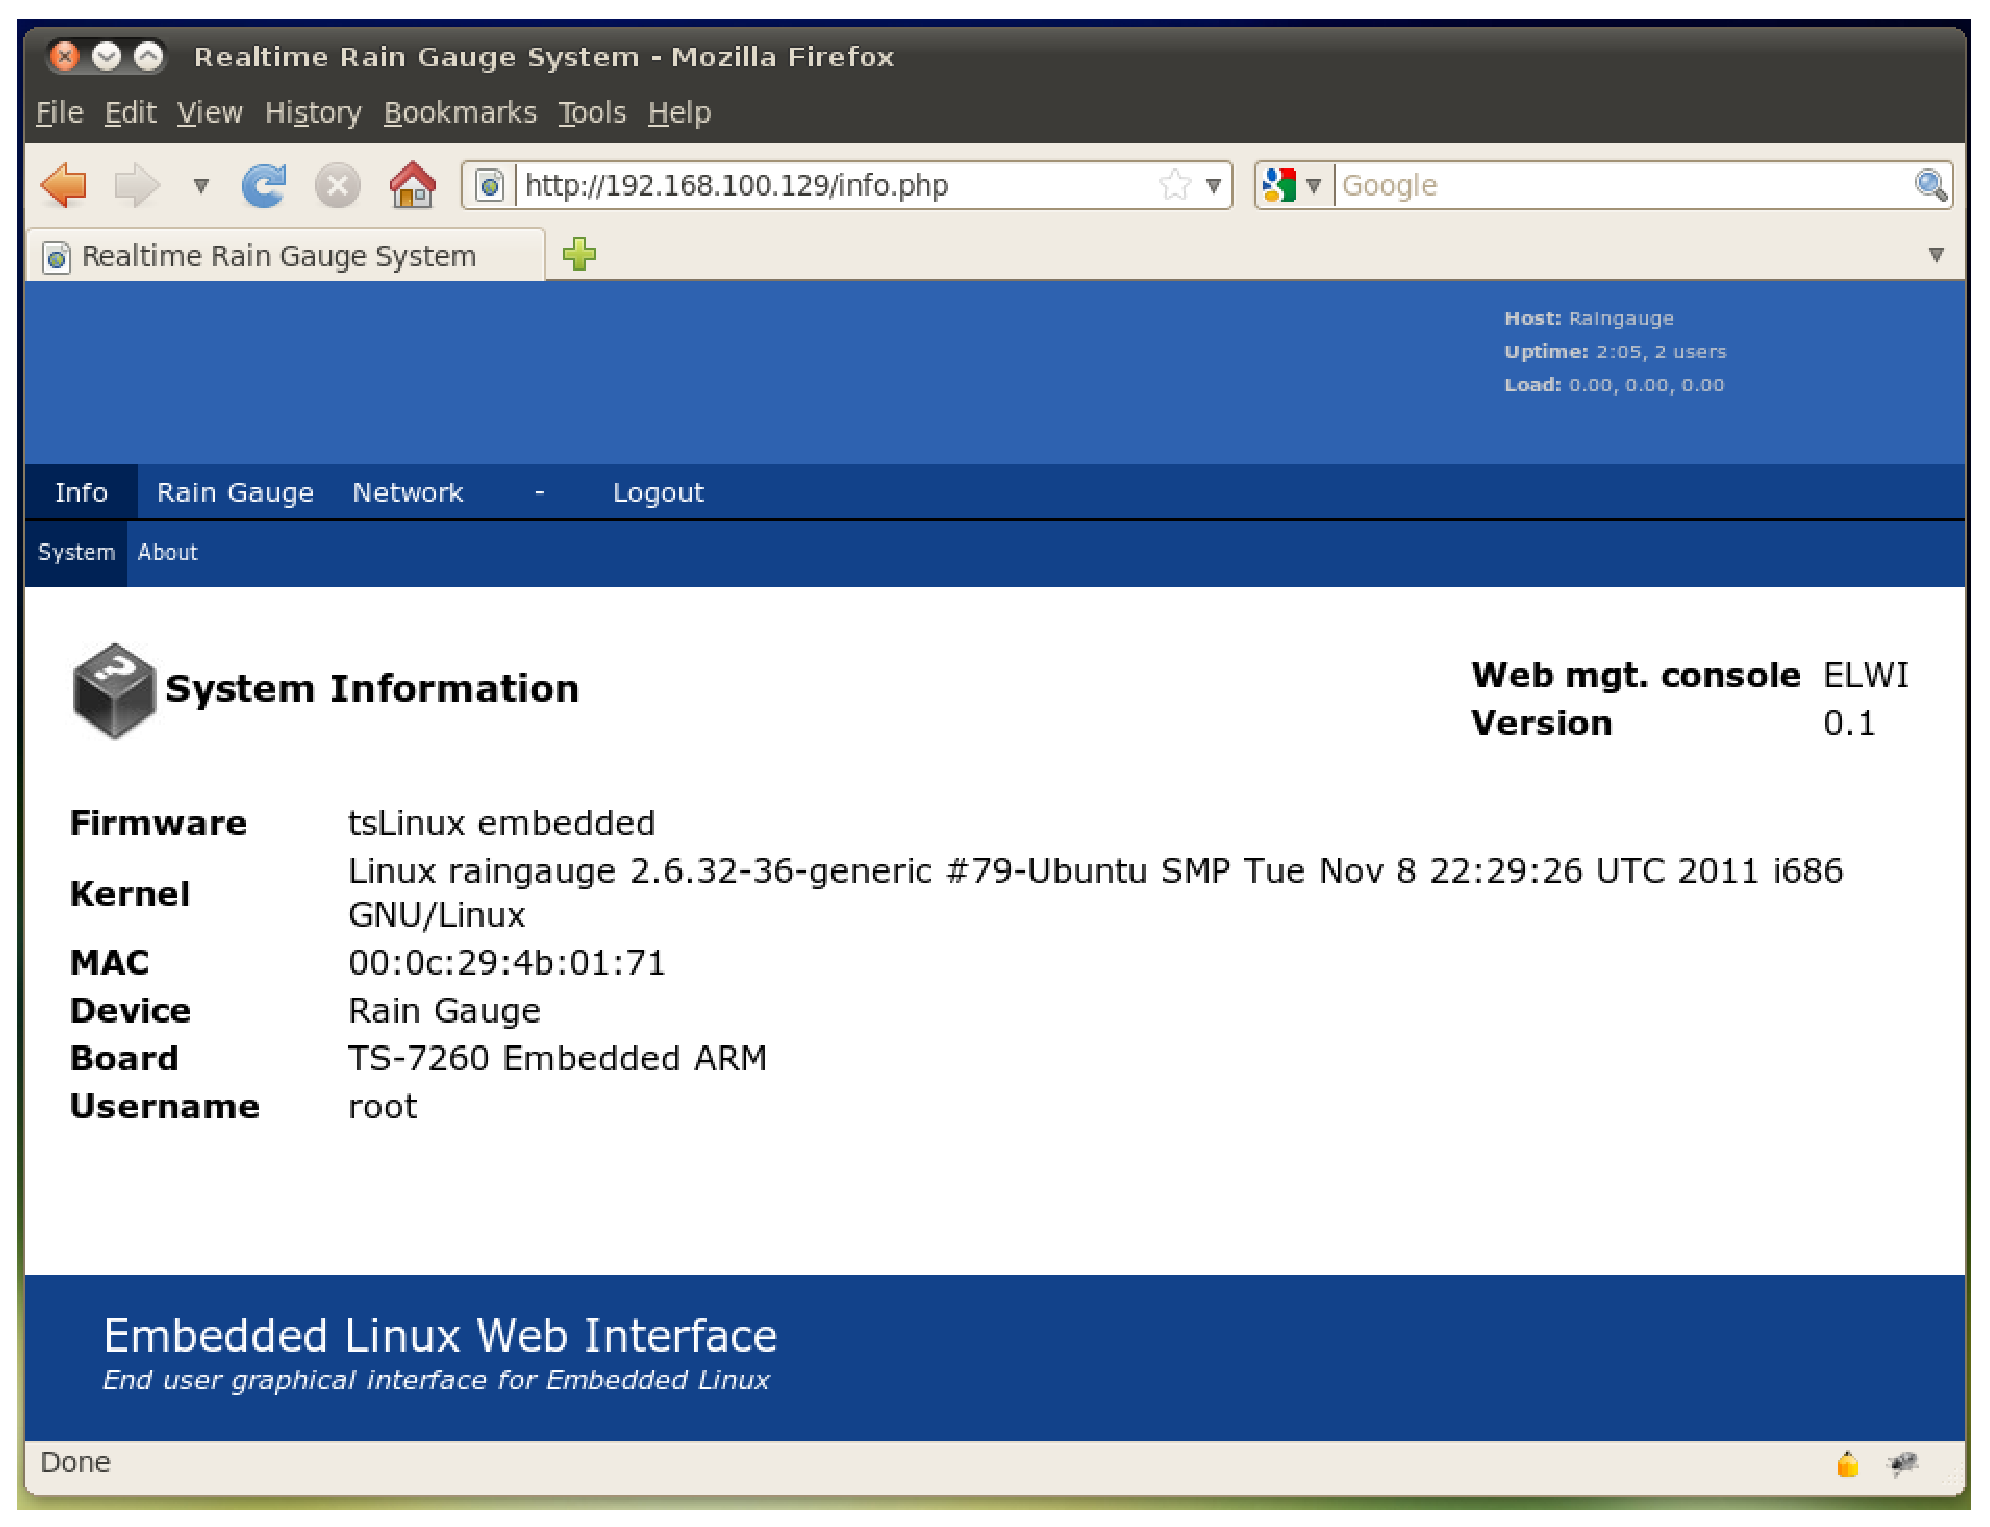
\includegraphics[width=0.75\textwidth]{source/fig/system-info.eps}}
\caption[Antaramuka maklumat umum sistem]{Antaramuka maklumat umum sistem}
\label{c4:f3}
\end{figure}
\begin{figure}[H]
\centering{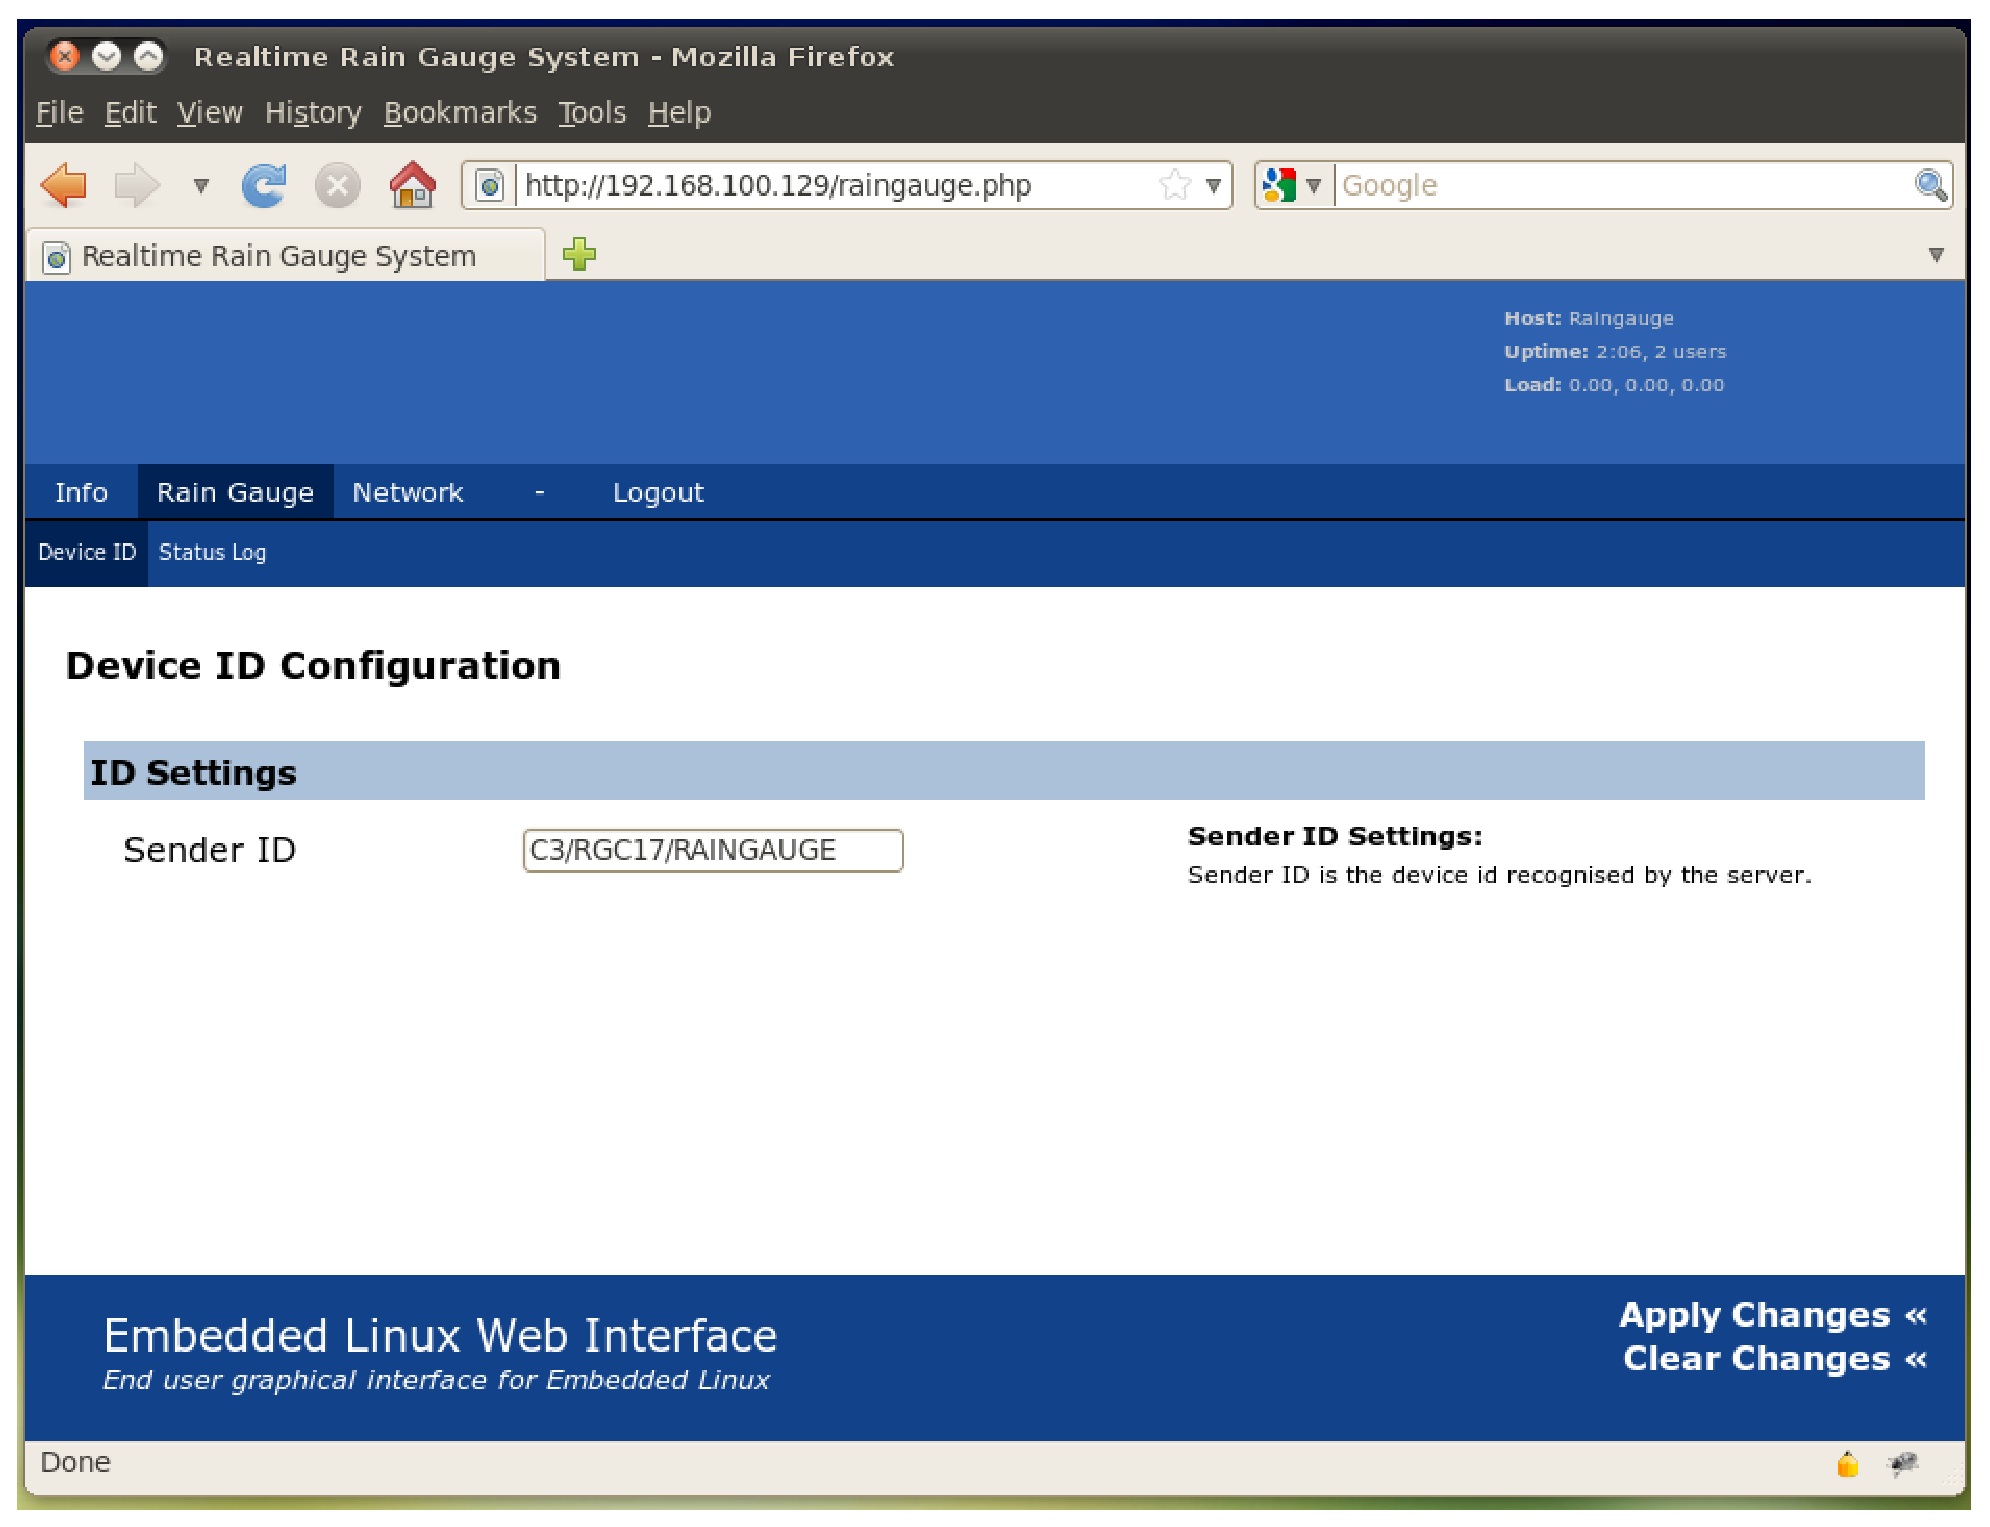
\includegraphics[width=0.75\textwidth]{source/fig/rg-dev-id.eps}}
\caption[Antaramuka konfigurasi ID rain gauge]{Antaramuka konfigurasi ID rain gauge}
\label{c4:f4}
\end{figure}
\begin{figure}[H]
\centering{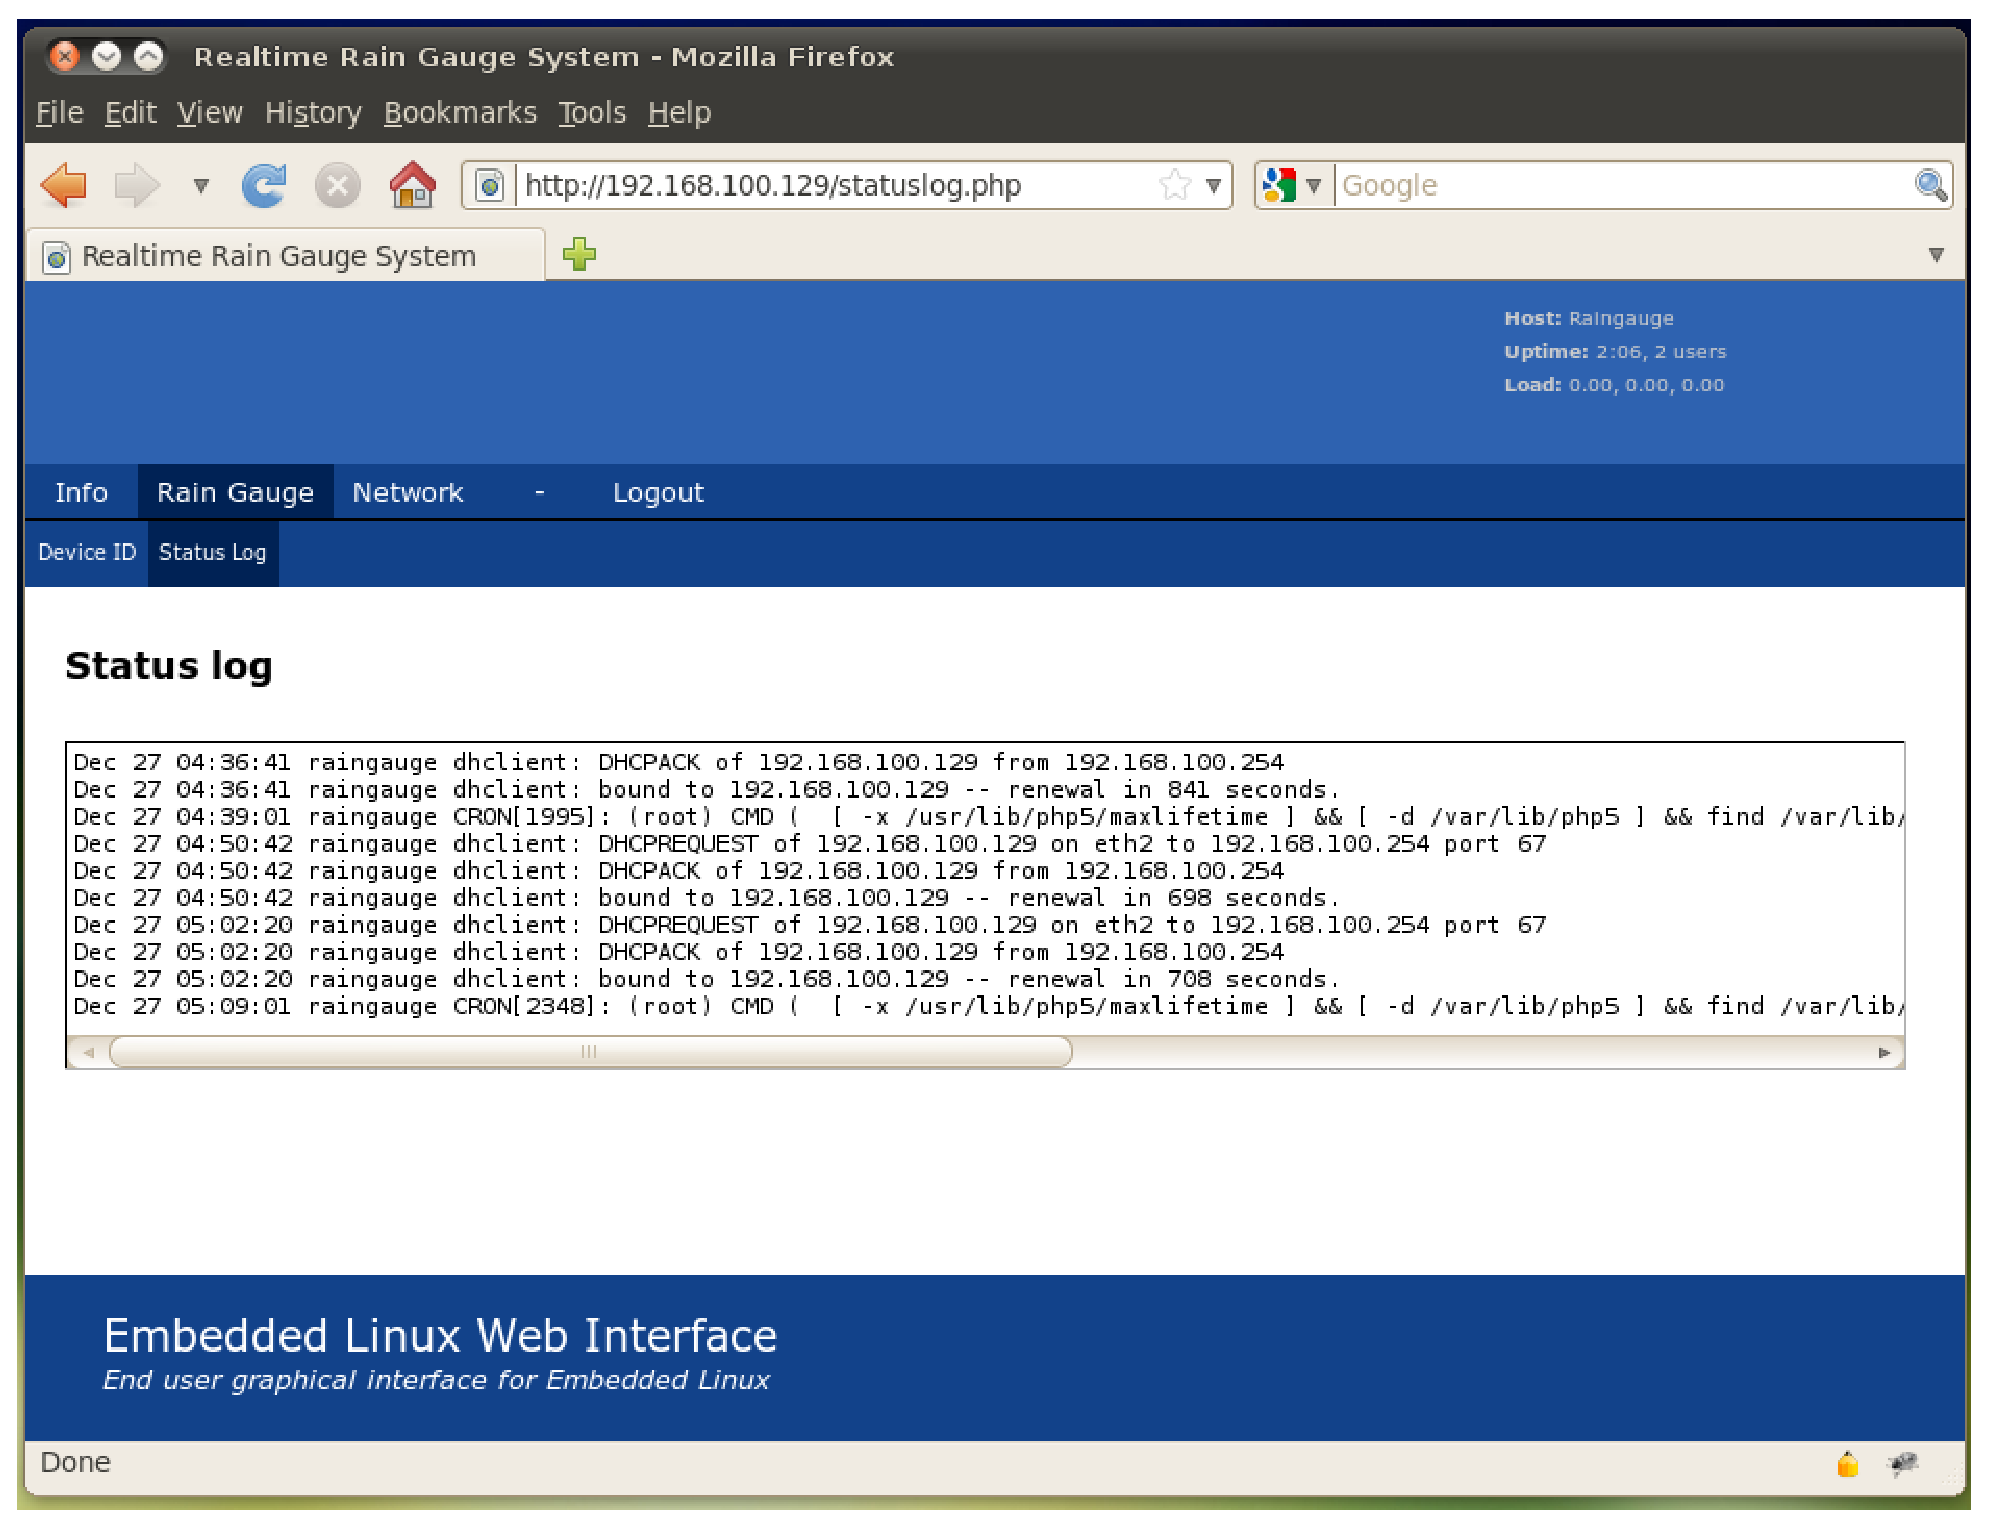
\includegraphics[width=0.75\textwidth]{source/fig/rg-status-log.eps}}
\caption[Antaramuka Log sistem terbenam]{Antaramuka Log sistem terbenam}
\label{c4:f5}
\end{figure}
\begin{figure}[H]
\centering{\includegraphics[width=0.75\textwidth]{source/fig/net-eth.eps}}
\caption[Antaramuka konfigurasi rangkaian]{Antaramuka konfigurasi rangkaian}
\label{c4:f6}
\end{figure}
\begin{figure}[H]
\centering{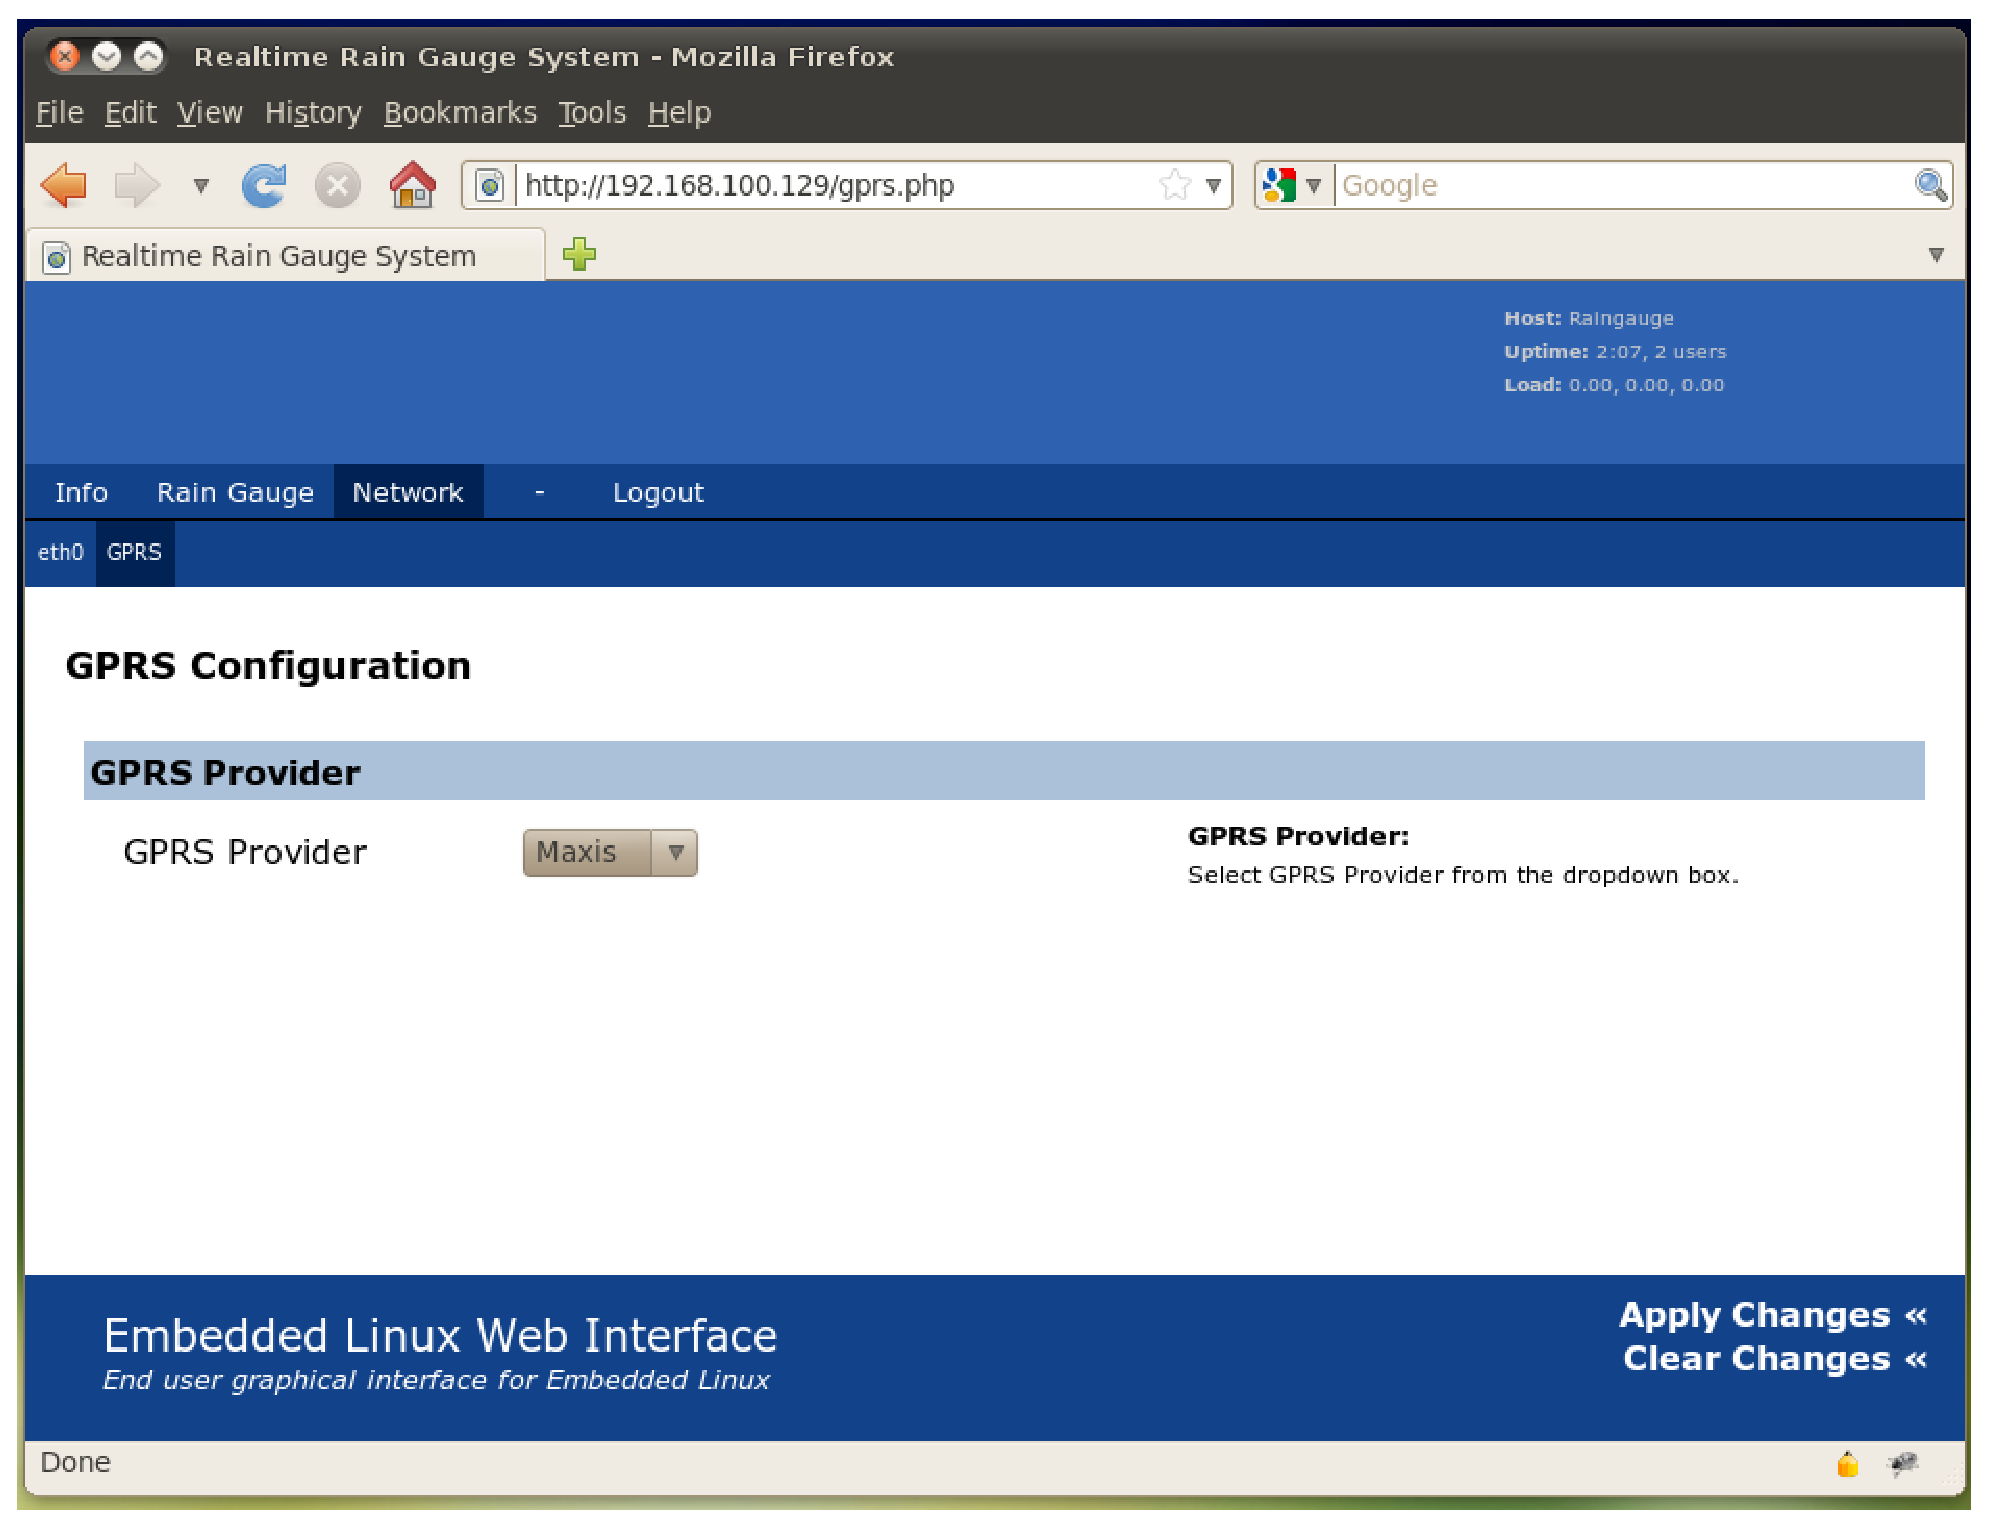
\includegraphics[width=0.75\textwidth]{source/fig/net-gprs.eps}}
\caption[Antaramuka konfigurasi GPRS]{Antaramuka konfigurasi GPRS}
\label{c4:f7}
\end{figure}

\section{Spesifikasi Input dan Output}
Semasa proses rekabentuk, spesifikasi input dan output dapat dikenalpasti. Untuk aplikasi ini, terdapat empat fungsi utama untuk aktiviti khusus yang ingin dilakukan iaitu untuk melihat status sistem, membuat tetapan rangkaian, membuat tetapan rain gauge, dan melihat log masa nyata.

\subsection{Spesifikasi Input}

\subsection{Spesifikasi Output}

\section{Kesimpulan}
Rekabentuk merupakan suatu fasa kritikal dalam proses pembangunan
aplikasi. Proses rekabentuk ini melibatkan kepelbagaian teknik, kaedah,
proses, aplikasi yang terlibat dan lain-lain proses rekabentuk yang berkaitan
sebagai langkah permulaan implementasi aplikasi yang bakal dibangunkan.
Kegagalan merekabentuk keperluan dan proses terlibat akan menyukarkan
proses atau fasa berikutnya.


